\documentclass{beamer}
\usepackage[utf8]{inputenc}
\usepackage{amsmath}
\usepackage{amsfonts}
\usepackage{amssymb}
\usepackage{amsthm}
\usepackage[russian]{babel}
\usepackage{hyperref}
\usepackage{enumerate}
\usepackage{graphicx}
\usepackage{float}
\usepackage{wrapfig}
\usepackage{natbib}
\usepackage{bibentry}
\usepackage{url}
\usetheme{Madrid}
\usecolortheme{crane}
\useinnertheme{rounded}
\usefonttheme{serif}
\setbeamertemplate{enumerate items}[default]
\addtobeamertemplate{frametitle}{
   \let\insertframetitle\insertsectionhead}{}
\addtobeamertemplate{frametitle}{
    \let\insertframesubtitle\insertsubsectionhead}{}

\makeatletter
  \CheckCommand*\beamer@checkframetitle{\@ifnextchar\bgroup\beamer@inlineframetitle{}}
  \renewcommand*\beamer@checkframetitle{\global\let\beamer@frametitle\relax\@ifnextchar\bgroup\beamer@inlineframetitle{}}
\makeatother

\begin{document}
\title{Строение рассеянных скоплений}
\author{Фархутдинова~А.~М. \and Кочергина~П.~B. \and Дромашко~M.~C.}
\institute{Санкт-Петербургский государственный университет}
\date{14 марта 2024}
\maketitle
\section*{Содержание}
\begin{frame}
    \tableofcontents
\end{frame}
\section{Важность изучения РЗС}
\begin{frame}
    \textbf{Рассеянное скопление} --- это тип звездного скопления, состоящего из~десятков или~нескольких тысяч звезд, 
    образовавшихся из~одного гигантского молекулярного облака и~имеющих примерно одинаковый возраст.
    \begin{figure}
        \centering
        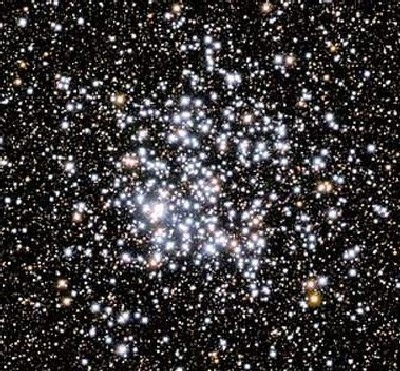
\includegraphics[width=0.4\textwidth]{pictures/РЗС.jpg}
    \end{figure}
\end{frame}
\begin{frame}
    Отличительной особенностью РЗС является то, что они представляют собой группы звезд, которые:
    \begin{itemize}
        \item Находятся от нас на практически одинаковом расстоянии
        \item Одинаково подвержены эффектам межзвездного поглощения и покраснения света
        \item Имеют почти одинаковый возраст
        \item Имеют практически идентичный химический состав и, как следствие, металличность
    \end{itemize}
    Рассеянные скопления являются ключевыми объектами в~изучении звездной эволюции. Поскольку члены скопления имеют одинаковый возраст и химический состав, 
    их свойства (такие как расстояние, возраст, металличность, поглощение и скорость) определить легче, 
    чем для изолированных звезд.
\end{frame}

    \section{История}

    \begin{frame}
        Некоторые РЗС известны с~древности.
        \begin{itemize}
            \item Плеяды известны еще со времен античности
            \item Греческий астроном Клавдий Птолемей упоминал Ясли, Двойное скопление в Персее и Скопление Птолемея
            \item Персидский астроном Ас-Суфи описал скопление Омикрон~Парусов
        \end{itemize}
    Тем не менее, различить их на~звезды смогли только после изобретения телескопа.
    \end{frame}
    \begin{frame}
        \begin{figure}
            \centering
            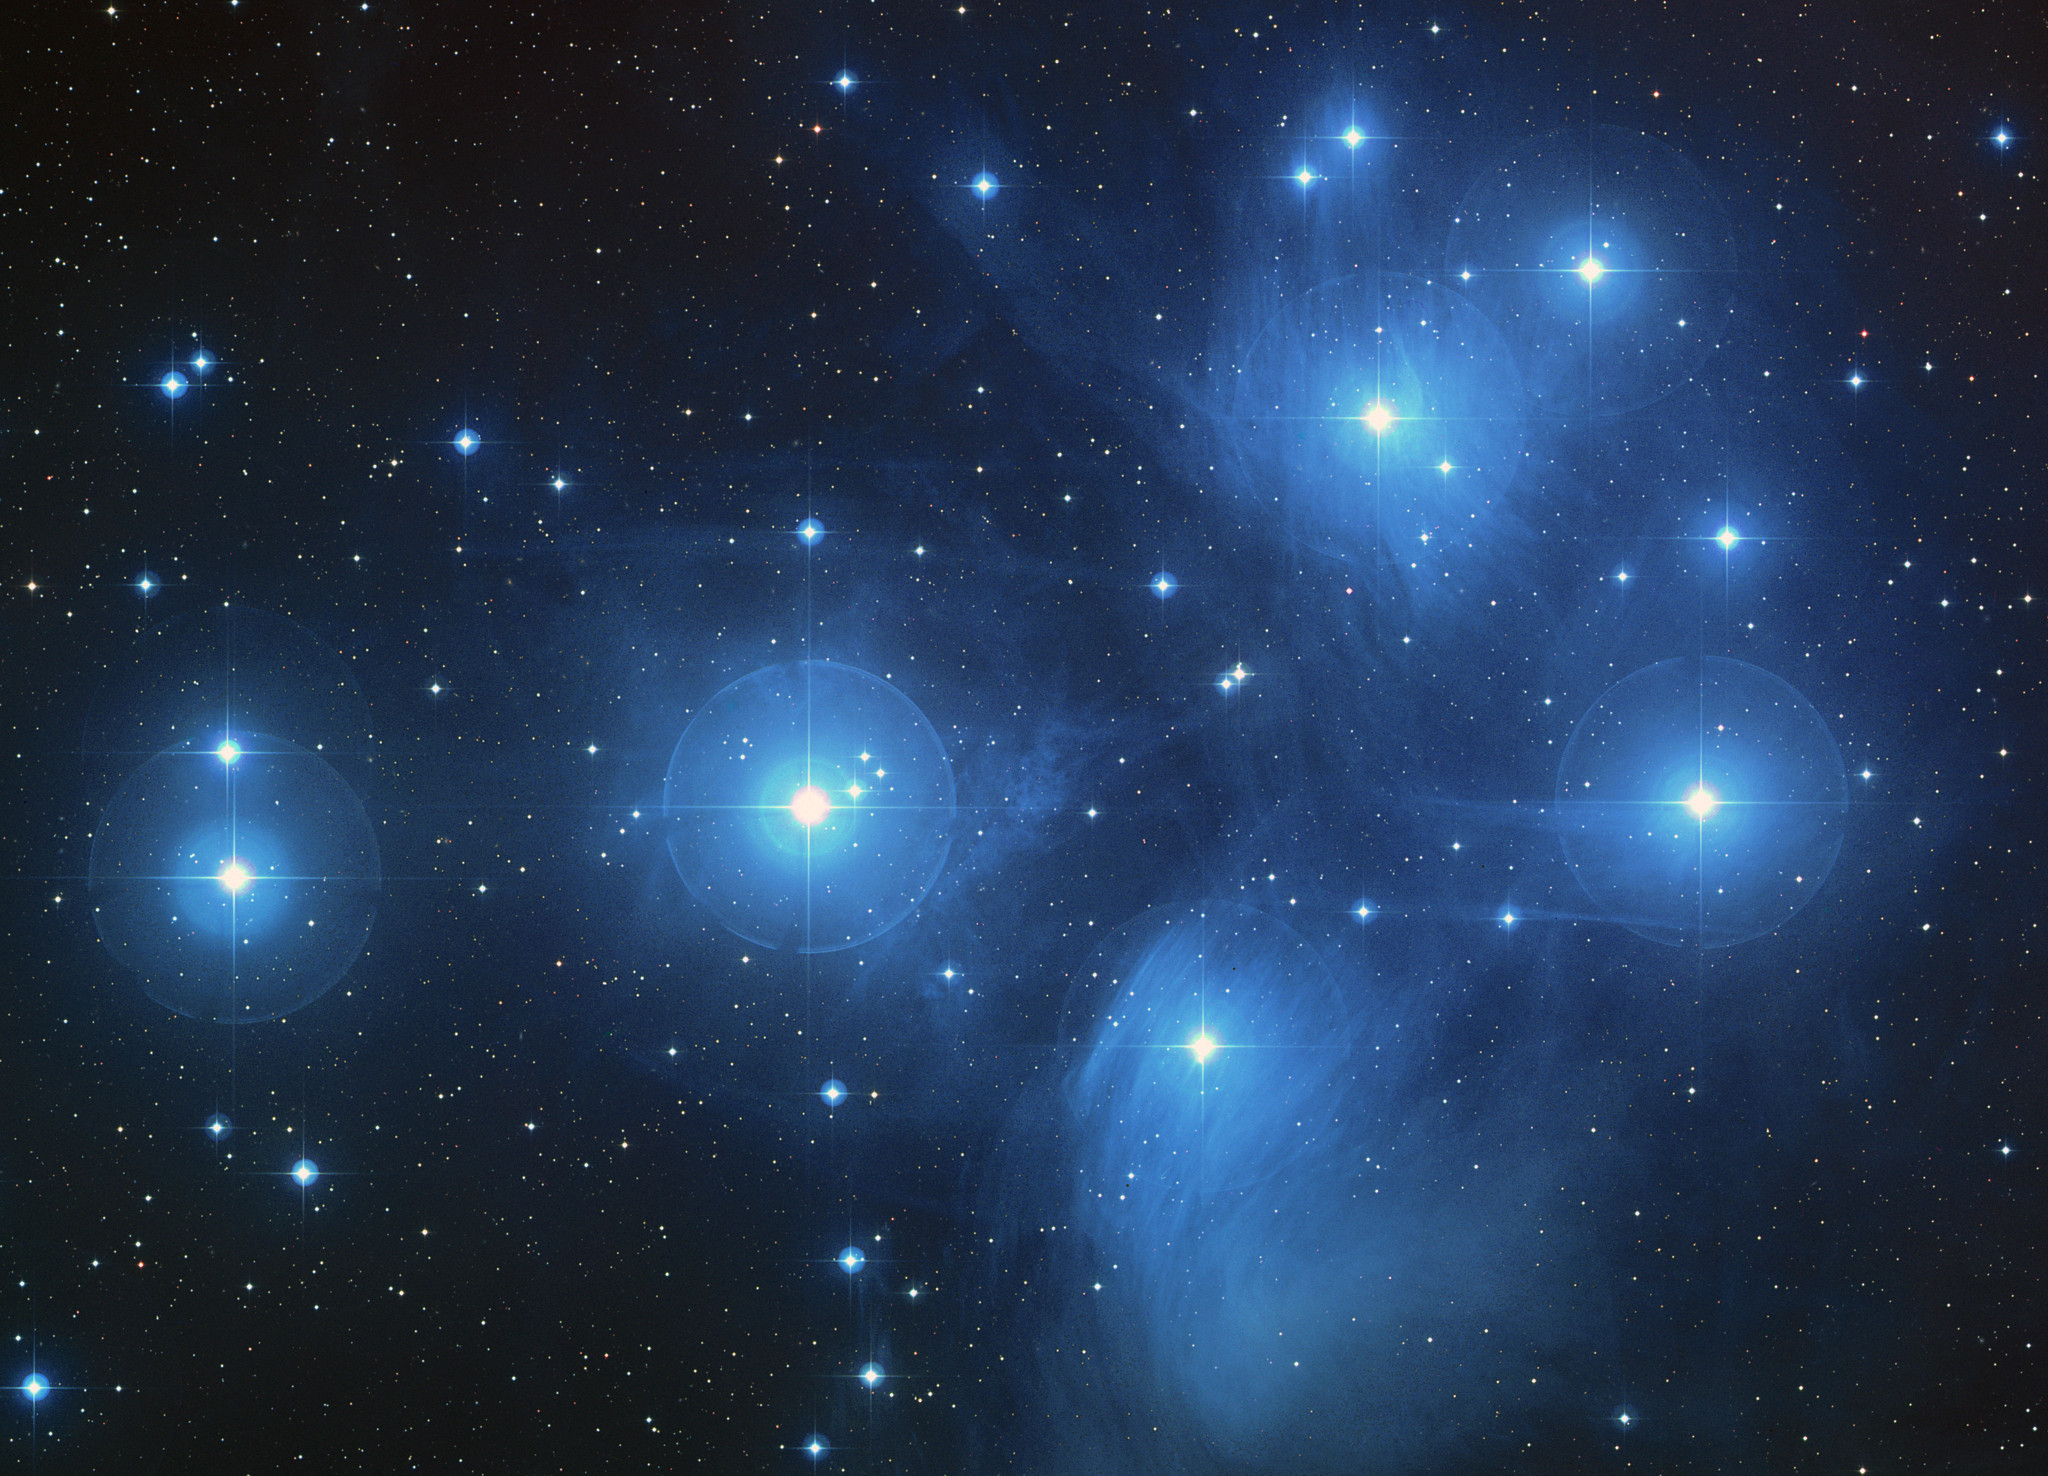
\includegraphics[width=0.7\textwidth]{pictures/Pl.jpg}
            \caption{Скопление Плеяд}
        \end{figure}
    \end{frame}
    \begin{frame}
        \begin{figure}
            \centering
            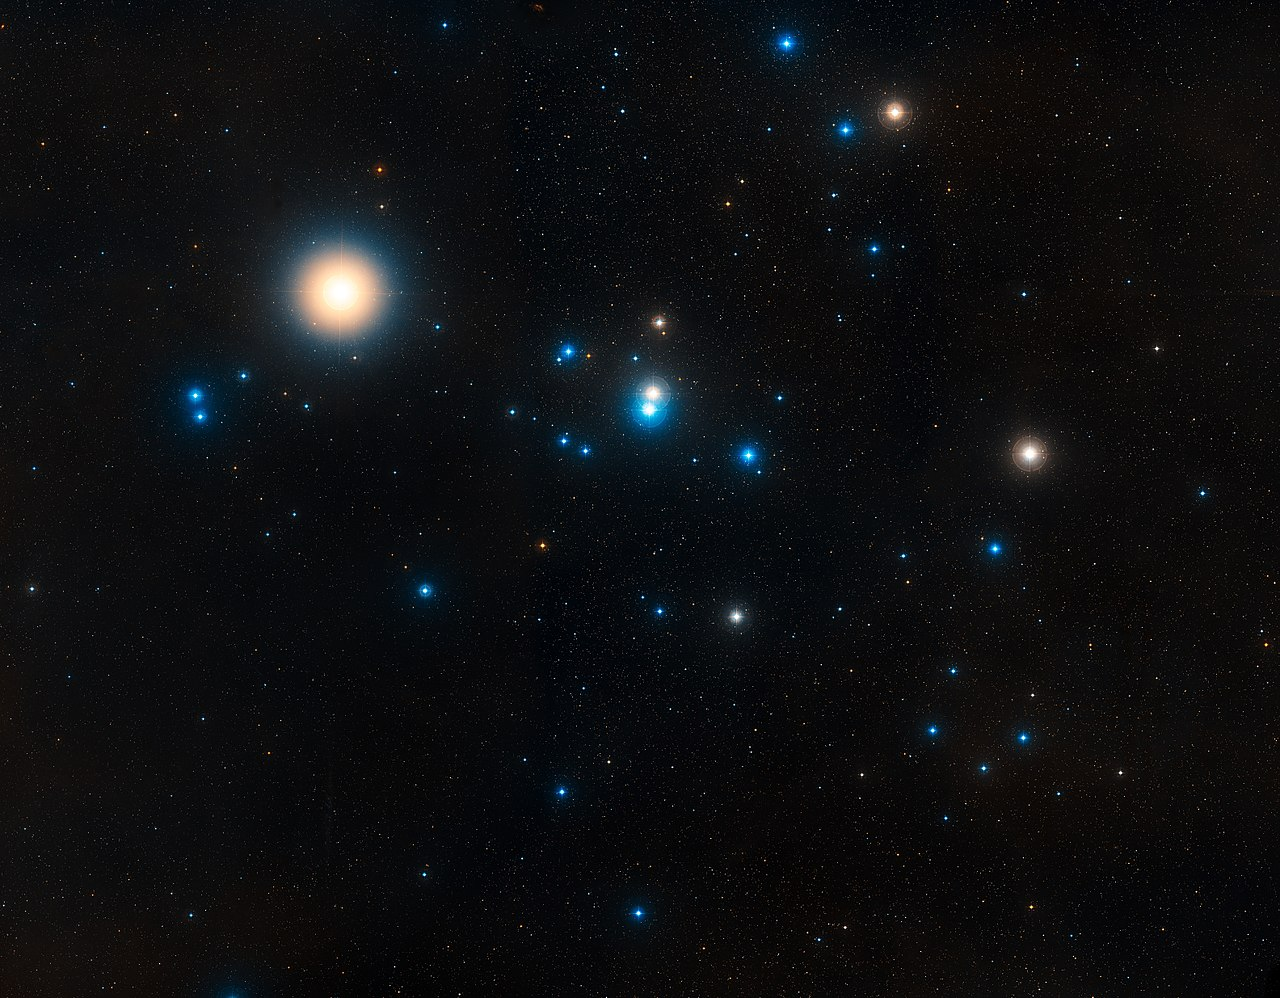
\includegraphics[width=0.7\textwidth]{pictures/Hyades.jpg}
            \caption{Скопление Гиад}
        \end{figure}
    \end{frame}

    \begin{frame}
        \begin{figure}
            \centering
            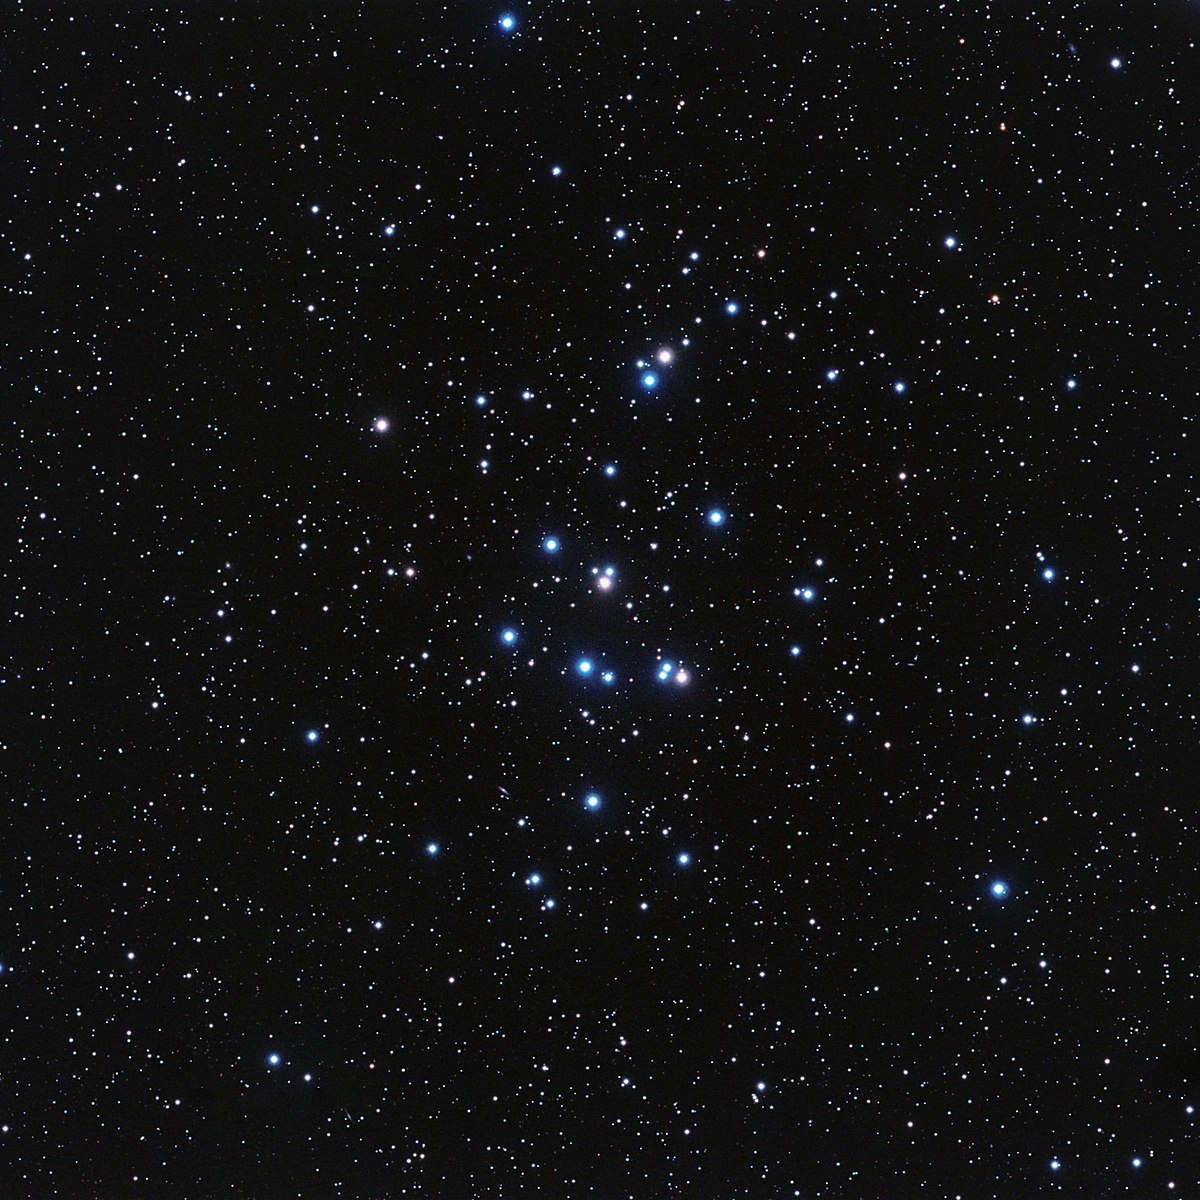
\includegraphics[width=0.5\textwidth]{pictures/yasli.jpg}
            \caption{Скопление Ясли}
        \end{figure}
    \end{frame}
    \begin{frame}
        \begin{itemize}
            \item Галлилей в~1609~г. обнаружил, что некоторые из~РЗС описанных Птолемеем являются группами из~большого числа звезд
            \item Джованни Годиерна в~1654~г. обнаружил M41, M47, NGC 2362 и NGC 2451
            \item 1774--1781~гг. --- публикация каталогов Шарля Мессье
            \item 1789~г. --- Ульям Гершель начинает всесторонне исследование <<туманных>> небесных обьектов
            \item 1888~г. --- публикация каталога NGC
        \end{itemize}
        Телескопические наблюдения позволили выявить два разных типа скоплений --- шаровые и рассеянные.
    \end{frame}
    \begin{frame}
        \large
        \begin{itemize}
            \item Эдуард Шёнфельд произвел первые микрометрические измерения позиций звезд в скоплениях в 1877~г.
            \item Адриан ван Маанен в 1918~г. смог измерить собственное движение звезд для части скопления Плеяд
            \item Первые диаграммы <<цвет—светимость>> для рассеянных скоплений были опубликованы Эйнаром Герцшпрунгом в~1911~г. вместе со схемами Плеяд и Гиад
        \end{itemize}
    \end{frame}


    %-------------------------------------------------------------------------------------
    \section{Особенности строения}
    \begin{frame}
        \Large
        \begin{itemize}
            \item Число звезд $\sim 10 \div 10^4$
            \item Как правило, состоят из~хорошо отличимого плотного ядра, окруженного более рассеянной <<короной>> из~звёзд
            \item Диаметр ядра $\sim 1$~пк
            \item Диаметр <<короны>> $\sim 10$~пк
            \item Плотность звезд в центре $\sim 40$~звезд/пк$^3$
        \end{itemize}
    \end{frame}
    \begin{frame}
        Иллюстрация из статьи\cite{AAA}
        \begin{figure}
            \centering
                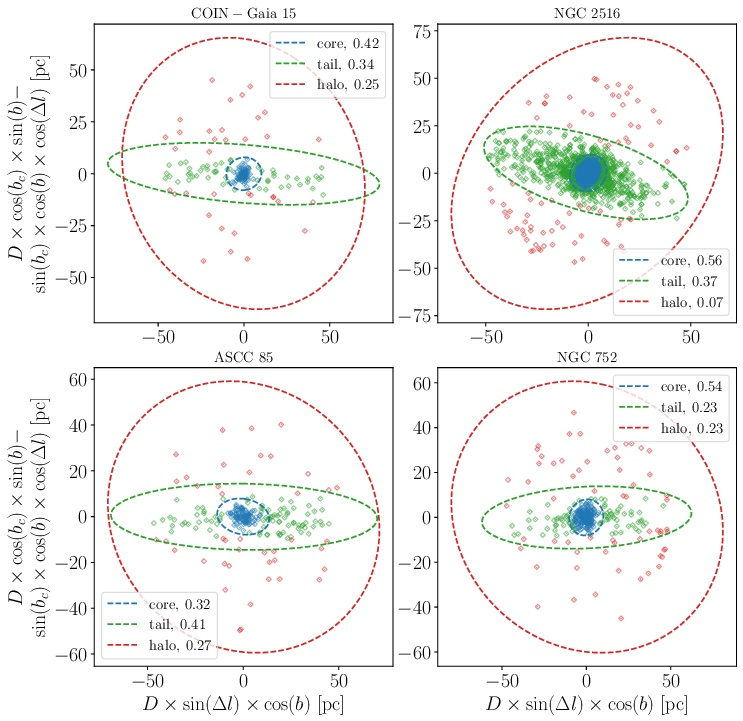
\includegraphics[width=0.4\textwidth]{pictures/Class1.jpg}
                \caption{Example of four clusters for which we detect a tidal tail. The blue, green, and red ellipses represent the 3$\sigma$ ellipse fit on the distribution of the stars standing for the core, 
                the tidal tail, and the halo, respectively. 
                The stars are colored according to which components they most likely belong. 
                The relative weights of each component are indicated in each panel.}
        \end{figure}
    \end{frame}
    \subsection*{Туманности}
    \begin{frame}
        Вместе со скоплением иногда наблюдается туманность. Сами туманности разделяют на два типа:
        \begin{itemize}
            \item Диффузная (светлая) туманность --- туманность излучающая свет, имеет три подтипа:
            \begin{enumerate}
                \item Эмиссионная (самосветящаяся) туманность --- межзвёздное облако, излучающее в оптическом диапазоне из-за ионизации собственного газа
                \item Отражательная туманность --- туманность (газово-пылевое облако), подсвечиваемая звездой
                \item Остаток сверхновой
            \end{enumerate}
            \item Темная туманность
        \end{itemize}
    \end{frame}
    \begin{frame}
        Тройная туманность (каталогизированная как Мессье 20 или M20 и NGC 6514 ) представляет собой рассеянное скопление,
        а также комбинацию Эмиссионной, Отражательной и Темной туманностей, расположенное в области Стрельца Млечного Пути.
        \begin{figure}
            \centering
            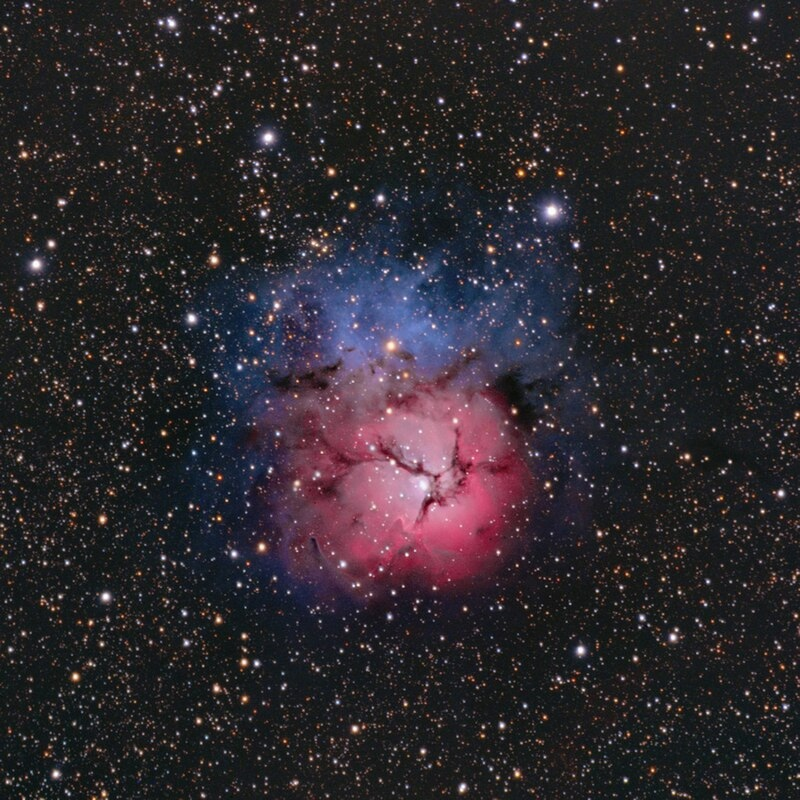
\includegraphics[width=0.4\textwidth]{pictures/Nebula.jpg}
        \end{figure}
    \end{frame}
    \section{Классификация Трамплера}
    \begin{frame}
        Схема классификации, предложенная Трамплером\cite{TrumpClass}. Состоит из трех частей.
        \begin{itemize}
            \item Концентрация
                \begin{enumerate}[I ---]
                    \item Отделено от поля; сильная концентрация к центру
                    \item Отделено от поля; слабая концентрация к центру
                    \item Отделено от поля; нет концентрации к центру
                    \item Плохо отделено от окружающего звездного поля
                \end{enumerate}
            \item Диапазон яркости
                \begin{enumerate}[1 ---]
                    \item Небольшой диапазон яркости
                    \item Умеренный диапазон яркости
                    \item Большой диапазон яркости
                \end{enumerate}
            \item Богатство
                \begin{enumerate}
                    \item[p ---] Бедное (меньше $50$ звезд)
                    \item[m ---] Умеренно богатое (от $50$ до $100$ звезд)
                    \item[r ---] Богатое (более $100$ звезд)
                \end{enumerate}
        \end{itemize}
        Буква «n» после класса Трамплера указывает на то, что со~скоплением связана туманность.
    \end{frame}
    %-------------------------------------------------------------------------------------

    \section{Методы отделения звезд скопления от звезд поля}
    \subsection{Кинематический метод}
    \begin{frame}
        Применяется если звезды скопления имеют сильно отличающиеся собственные скорости от~скоростей звезд фона. 
        \begin{figure}
            \centering
            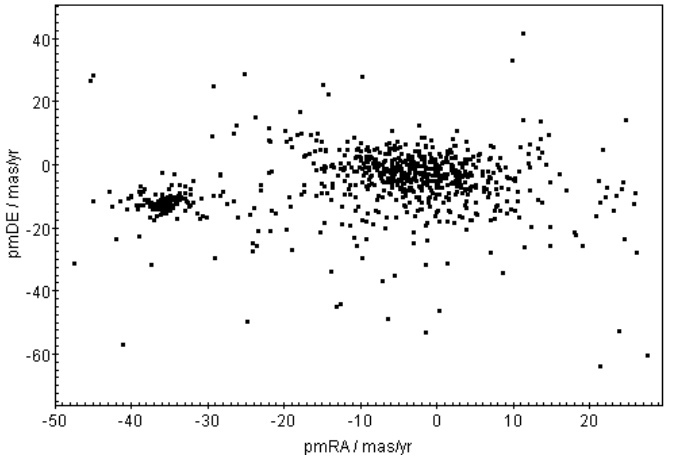
\includegraphics[width=0.5\textwidth]{pictures/Kin.jpg}
            \caption{Поле движения звезд в поле скопления Ясли}
        \end{figure}
        К сожалению, случаи такого разделения редки.
    \end{frame}
    \subsection{Статистический метод Сандерса}
    \begin{frame}
        Метод предложенный Сандерсом\cite{Sanders}. Позволяет определить
        \begin{itemize}
            \item Cредние собственные движения звезд скопления $\mu = (\mu_\alpha, \mu_\delta)$
            \item Cредние собственные движения звезд фона $\mu^f = (\mu^f_\alpha, \mu^f_\delta)$
            \item Cредние дисперсии собственных движений звезд скопления $\sigma = (\sigma_\alpha, \sigma_\delta)$
            \item Cредние дисперсии собственных движений звезд фона $\sigma^f = (\sigma^f_\alpha, \sigma^f_\delta)$
            \item Относительное количество звезд в скоплении $N$
            \item Вероятность принадлежности звезды к скоплению $P$
        \end{itemize}
    \end{frame}
    \begin{frame}
        \begin{itemize}
            \item Составляется выборка звезд известными собственными движениями $(\mu^i_\alpha, \mu^i_\delta)$ и их погрешностями $(\varepsilon^i_\alpha, \varepsilon^i_\delta)$
            \item Составляется функция плотности вероятности для звезд скопления
            \scriptsize
            \begin{equation*}
                    F_i(\mu, \sigma, N) = \cfrac{N}{2\pi\sqrt{\sigma^{2}_\alpha + \varepsilon_\alpha^{i^2}}\sqrt{\sigma^{2}_\delta + \varepsilon_\delta^{i^2}}}\exp\left(-0.5\left[ \cfrac{(\mu^i_\alpha - \mu_\alpha)^2}{\sigma^{2}_\alpha + \varepsilon_\alpha^{i^2}} + \cfrac{(\mu^i_\delta - \mu_\delta)^2}{\sigma^{2}_\delta + \varepsilon_\delta^{i^2}} \right]\right)
            \end{equation*}

            \normalsize и для звезд фона вида
            \scriptsize
            \begin{equation*}
                    F^f_i(\mu^f, \sigma^f, N) = \cfrac{1-N}{2\pi\sqrt{\sigma^{f^2}_\alpha + \varepsilon_\alpha^{i^2}}\sqrt{\sigma^{f^2}_\delta + \varepsilon_\delta^{i^2}}}\exp\left(-0.5\left[ \cfrac{(\mu^i_\alpha - \mu^f_\alpha)^2}{\sigma^{f^2}_\alpha + \varepsilon_\alpha^{i^2}} + \cfrac{(\mu^i_\delta - \mu^f_\delta)^2}{\sigma^{f^2}_\delta + \varepsilon_\delta^{i^2}} \right]\right)
            \end{equation*}
        \end{itemize}
    \end{frame}
    \begin{frame}
        \begin{itemize}
            \item Составляется функция правдоподобия
            \begin{equation*}
                Q(\mu, \sigma, \mu^f, \sigma^f, N) = \prod_i \left(F_i + F^f_i\right)
            \end{equation*}
            Ее максимум дает нам значения $\mu$, $\sigma$, $\mu^f$, $\sigma^f$, $N$
            \item Вероятность принадлежности звезды выборки $i$ к скоплению оценивается как 
            \begin{equation*}
                P_i = \cfrac{F_i}{F_i + F^f_i}
            \end{equation*}
        \end{itemize}
    \end{frame}
    \begin{frame}
        \begin{figure}
            \centering
            \includegraphics[width=0.7\textwidth]{pictures/Sansan.jpg}
        \end{figure}
    \end{frame}
    \section*{Параметры РЗС}
    \begin{frame}
        \begin{figure}
            \centering
            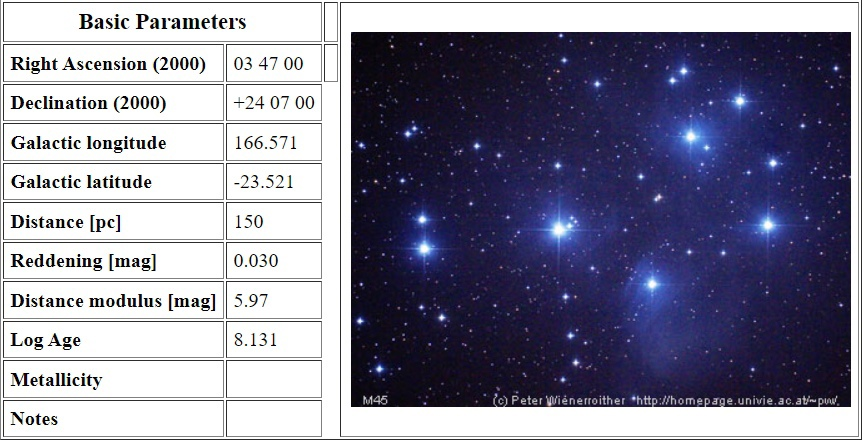
\includegraphics[width=0.9\textwidth]{pictures/Params.jpg}
        \end{figure}
    \end{frame}
    \section{Методы определения параметров РЗС}
    \subsection{Методы определения избытков цвета. Двухцветная диаграмма}
    \begin{frame}
        Основной способ определения избытка цвета РЗС.
        \begin{columns}
            % Column 1
            \begin{column}{0.5\textwidth}
                    \begin{itemize}
                        \item Типичная погрешность метода $\sim 0^m.01$
                        \item Избыток цвета определяется как сдвиг 
                            влево и вверх всей диаграммы скопления вдоль линии нарастающего покраснения до совпадения с последовательностью непокрасневших звёзд
                    \end{itemize}
            \end{column}
            % Column 2    
            \begin{column}{0.5\textwidth}
                \begin{figure}
                \centering
                    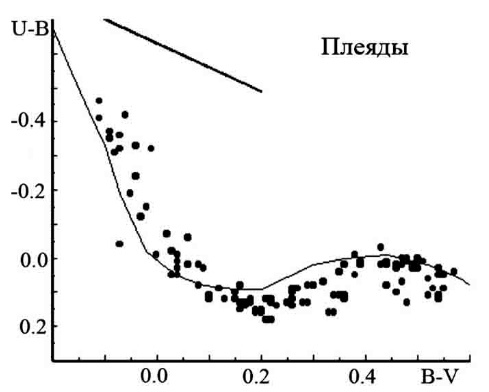
\includegraphics[width=0.9\textwidth]{pictures/Pl2Col.jpg}
                \end{figure}
            \end{column}
        \end{columns}
    \end{frame}
    \begin{frame}
        Применим не всегда.
        \begin{columns}
            % Column 1
            \begin{column}{0.5\textwidth}
                    \begin{itemize}
                        \item Всегда имеется трудность с~отделением членов скопления от~звёзд поля
                        \item У~заметного числа скоплений покраснения для разных звёзд не~равны --- имеется дифференциальное покраснение
                    \end{itemize}
            \end{column}
            % Column 2    
            \begin{column}{0.5\textwidth}
                \begin{figure}
                \centering
                    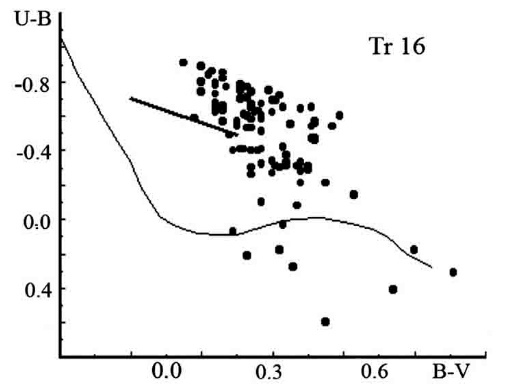
\includegraphics[width=0.9\textwidth]{pictures/Tr2Col.jpg}
                \end{figure}
            \end{column}
        \end{columns}
    \end{frame}
    \subsection{Методы определения избытков цвета. Q-метод}
    \begin{frame}
        В случае небольших покраснений, когда можно пренеберечь отличием линии нарастающего покраснения от прямой линии, 
        для определения индивидуальных избытков цвета можно применить Q-метод.
        \begin{itemize}
            \item Введем параметр $Q_{UBV} = (U-B) - K*(B-V)$, где $K$ --- наклон линии покраснения. 
            Эта величина не зависит от величины межзвездного покраснения
            \item Заменим двухцветную диаграмму на диаграмму $\left(B-V, Q_{UBV}\right)$
            \item На полученной диаграмме линии нарастающего покраснения --- прямые параллельные координатным осям
        \end{itemize}
        Таким образом существенно упрощается определение избытков цвета.
    \end{frame}

    \subsection{Методы определения расстояний. Метод НГП}
    \begin{frame}
        Зная диаграмму Герцшпрунга-Рассела скопления, можно определить истинный модуль расстояния до него. Для этого используют метод начальной главной последовательности.
        \begin{columns}
            % Column 1
            \begin{column}{0.6\textwidth}
                \begin{itemize}
                    \item Звезды скопления находятся почти на~одном и том же расстоянии от~Солнца
                    \item Если пренеберечь наличием сильно проэволюционировавших звезд, то можно считать, 
                    что диаграмма скопления совпадает с~главной последовательностью с~точностью до~сдвига
                    \item Относительная погрешность определения расстояний $\sim 20$\%
                \end{itemize}
            \end{column}
            % Column 2    
            \begin{column}{0.4\textwidth}
                \begin{figure}
                \centering
                    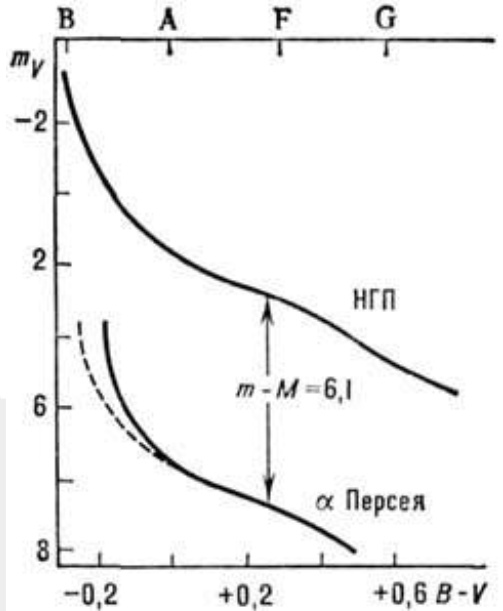
\includegraphics[width=0.6\textwidth]{pictures/NGP.jpg}
                \end{figure}
            \end{column}
        \end{columns}

    \end{frame}
    \subsection{Методы определения расстояний. Цефеиды}
    \begin{frame}
        В некоторых РЗС обнаружены желтые пульсирующие гиганты --- цефеиды, их можно использовать для определения расстояния до~скопления.
        \begin{columns}
            % Column 1
            \begin{column}{0.6\textwidth}
                \begin{itemize}
                    \item Цефеиды имеют хорошо изученную зависимость между периодом и светимостью, поэтому можно определить расстояние до~цефеиды
                    \item Поскольку расстояния звезд скопления до~Солнца почти равны, 
                    то расстояние до~цефеиды можно взять как оценку расстояния до~скопления
                \end{itemize}
            \end{column}
            % Column 2    
            \begin{column}{0.4\textwidth}
                \begin{figure}
                \centering
                    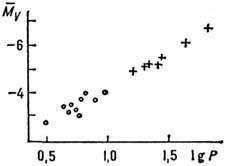
\includegraphics[width=0.7\textwidth]{pictures/Cep.jpg}
                \end{figure}
            \end{column}
        \end{columns}
    \end{frame}
    \subsection{Метод изохрон}
    \begin{frame}
        Изохрона --- линия равного возраста на~диаграмме <<цвет~---~звездная величина>>.
        \begin{columns}
            \begin{column}{0.5\textwidth}
                \begin{itemize}
                    \item Построение теоретических изохрон происходит при помощи численного расчета эволюционных треков звезд различных масс
                    \item Точность вычисления эволюционных треков звезд сильно падает на поздних эволюционных стадиях
                \end{itemize}
            \end{column}
            % Column 2    
            \begin{column}{0.5\textwidth}
                \begin{figure}
                \centering
                    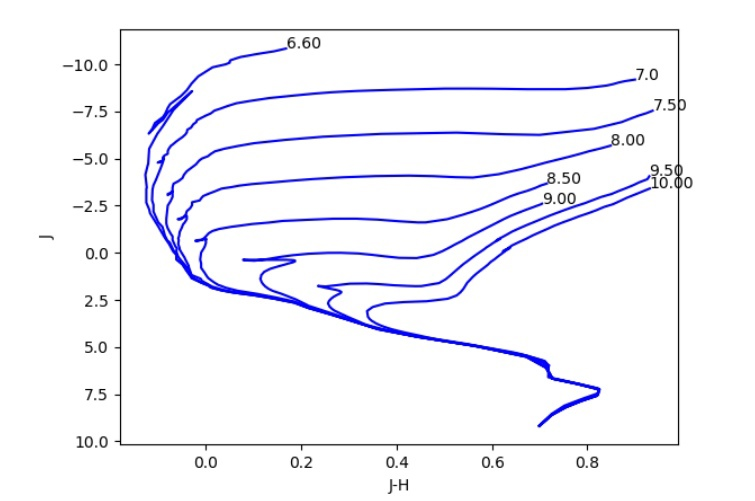
\includegraphics[width=0.9\textwidth]{pictures/isochrone.jpg}
                \end{figure}
            \end{column}
        \end{columns}
    \end{frame}
    \begin{frame}
        Метод заключается в совмещении диаграммы <<цвет~---~звездная величина>> скопления с~соответствующей изохроной:
        \begin{columns}
            \begin{column}{0.5\textwidth}
                \begin{figure}
                    \centering
                        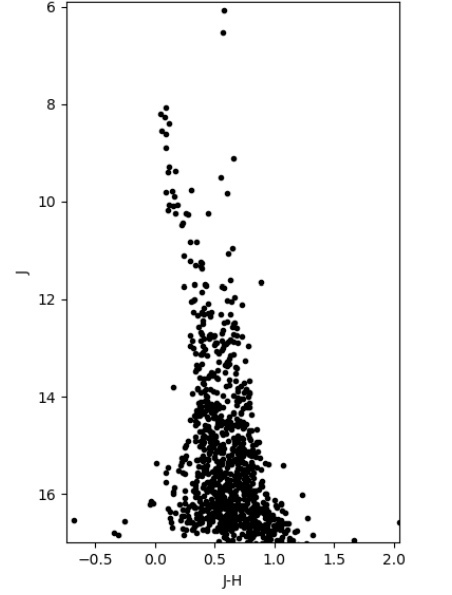
\includegraphics[width=0.7\textwidth]{pictures/Iso1.jpg}
                    \end{figure}
            \end{column}
            % Column 2    
            \begin{column}{0.5\textwidth}
                \begin{figure}
                \centering
                    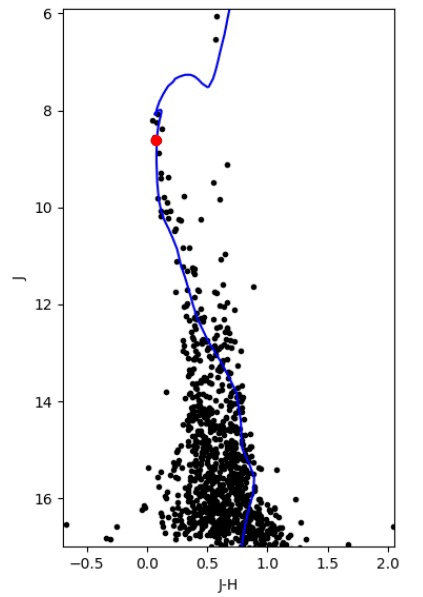
\includegraphics[width=0.65\textwidth]{pictures/Iso2.jpg}
                \end{figure}
            \end{column}
        \end{columns}
    \end{frame}
    \begin{frame}
        При этом одновременно определяются сразу три параметра скопления:
        \begin{columns}
            \begin{column}{0.5\textwidth}
                \begin{itemize}
                    \item Видимый модуль расстояния в~соответствующей полосе
                    \item Избыток соответствующего цвета
                    \item Возраст скопления
                \end{itemize}
            \end{column}
            % Column 2    
            \begin{column}{0.5\textwidth}
                \begin{figure}
                \centering
                    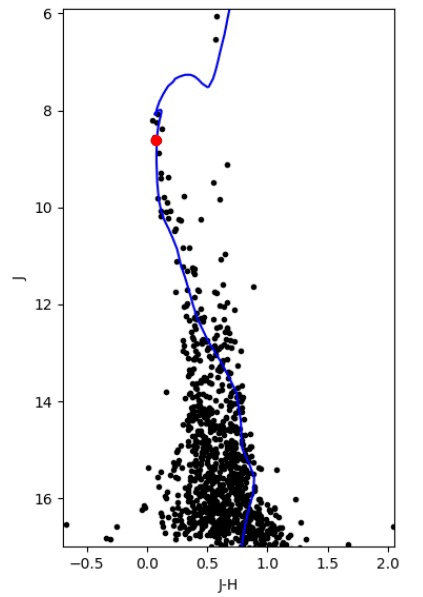
\includegraphics[width=0.5\textwidth]{pictures/Iso2.jpg}
                \end{figure}
            \end{column}
        \end{columns}
        Красная точка --- <<точка поворота>> ---  точка, где звезды сходят с главной последовательности после выгорания водородного топлива (самая <<голубая>>).
        Эта точка характеризует возраст скопления, позволяя подобрать нужную изохрону.
    \end{frame}
    \begin{frame}
        \begin{figure}
            \centering
                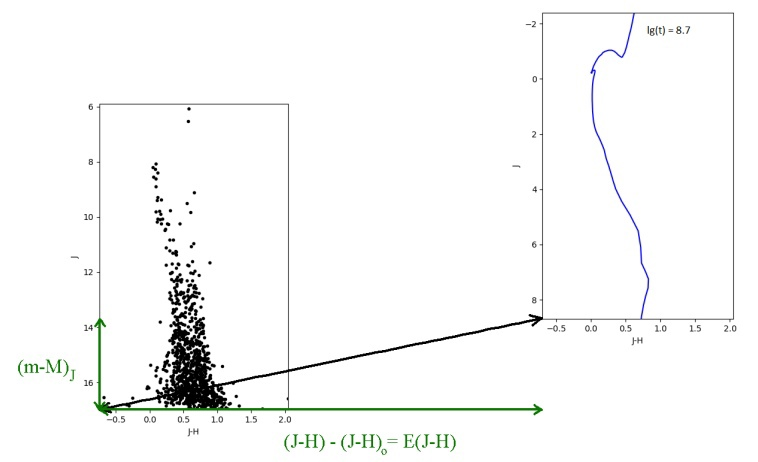
\includegraphics[width=0.8\textwidth]{pictures/Alsa.jpg}
            \end{figure}
    \end{frame}
    \subsection*{Метод изохрон. h-индекс}
    \begin{frame}
    В 2017~г. Дамбисом и др. было показано\cite{Dambis}, что подбор изохроны можно существенно упростить. 
    Для этого вводится величина $h = 0.755R + 0.245I - H_{\alpha}$, называемая h-индексом ($H_{\alpha}$ --- звездная величина в фильтре, центрированном по линии Бальмера).
    \begin{columns}
        \begin{column}{0.5\textwidth}
            \begin{itemize}
                \item h-индекс не зависит от покраснения (в первом приближении)
                \item Изохроны, построенные на диаграмме $\left(R-I, h\right)$ имеет минимум на одном и том же показателе цвета, 
                что позволяет сразу определить избыток цвета сдвигая диграмму скопления вдоль оси абсцисс
            \end{itemize}
        \end{column}
        % Column 2    
        \begin{column}{0.5\textwidth}
            \begin{figure}
            \centering
                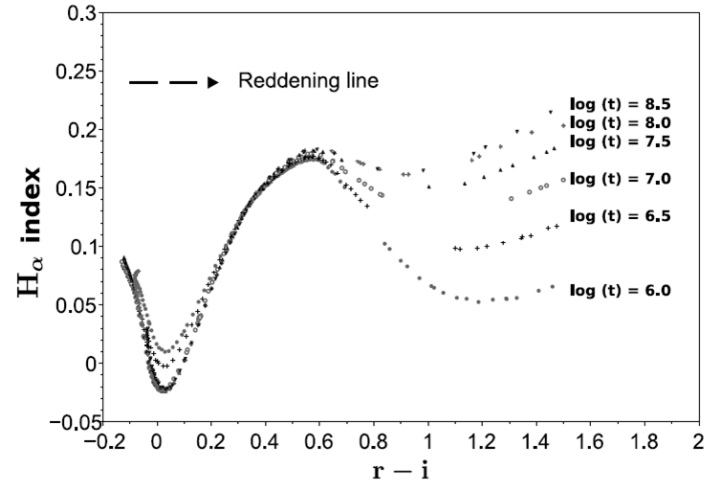
\includegraphics[width=0.8\textwidth]{pictures/Isoh.jpg}
            \end{figure}
        \end{column}
    \end{columns}
    \end{frame}
    \begin{frame}
        \begin{itemize}
        \item Аналогично диаграмме $\left(R-I, h\right)$, изохроны на диаграмме $\left(h, R\right)$ имеют минимум при одном и том же значении R, 
        что позволяет сдвигом вдоль координатной оси определить модуль расстояния
        \item Зная избыток цвета и модуль расстояния по диаграмме $\left(R-I, R\right)$ можно определить возраст
        \item На практике часто диаграмма $\left(h, R\right)$ оказывается неудовлетворительной, поэтому после определения избытка цвета
        сразу переходят к диаграмме $\left(R-I, R\right)$, подбирая сдвигом изохроны сразу два параметра
        \end{itemize}
    \end{frame}
    \begin{frame}
        \begin{columns}
            \begin{column}{0.333\textwidth}
                \begin{figure}
                    \centering
                    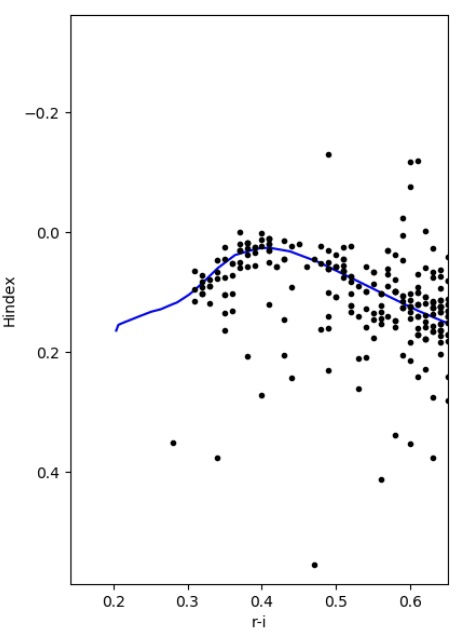
\includegraphics[width=0.8\textwidth]{pictures/Isoh1.jpg}
                \end{figure}
            \end{column}
            % Column 2    
            \begin{column}{0.333\textwidth}
                \begin{figure}
                    \centering
                    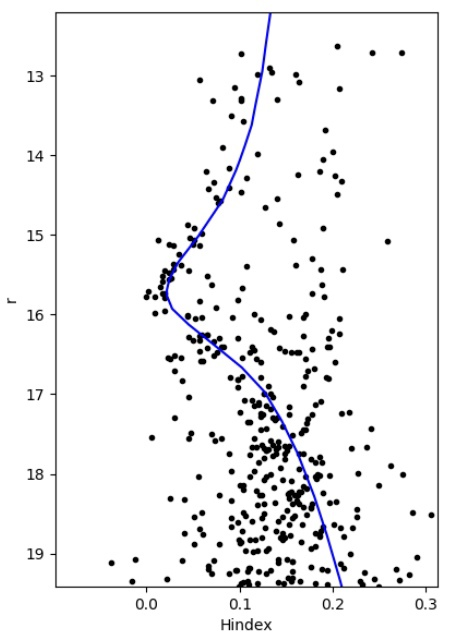
\includegraphics[width=0.8\textwidth]{pictures/Isoh2.jpg}
                \end{figure}
            \end{column}
            \begin{column}{0.333\textwidth}
                \begin{figure}
                    \centering
                    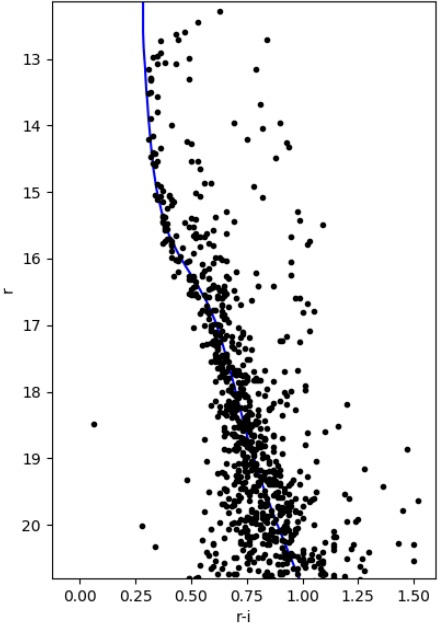
\includegraphics[width=0.75\textwidth]{pictures/Isoh3.jpg}
                \end{figure}
            \end{column}
        \end{columns}
    \end{frame}
    \subsection*{Метод изохрон}
    \begin{frame}
        Метод изохрон имеет ряд недостатков:
        \begin{itemize}
            \item Метод изохрон сильно зависит от~модели эволюции звезд, особенно велики расхождения в~области малых масс
            \item Так как самыми распространенными звездами являются K гиганты и A карлики, 
            может возникнуть псевдо главная последовательность или другие ложные особенности, что затруднит определение параметров скопления
            \item Для точных результатов нужно хорошо изучить поглащение в поле скопления
        \end{itemize}
    \end{frame}

    %-------------------------------------------------------------------------------------
    \section{Звездные ассоциации}
    \begin{frame}
        \textbf{Звёздные ассоциации} --- группировки гравитационно несвязанных или слабо связанных звёзд. 
        Такие звёзды имеют общее происхождение и довольно молоды: их возраст не превышает нескольких десятков миллионов лет.
        \begin{figure}
            \centering
            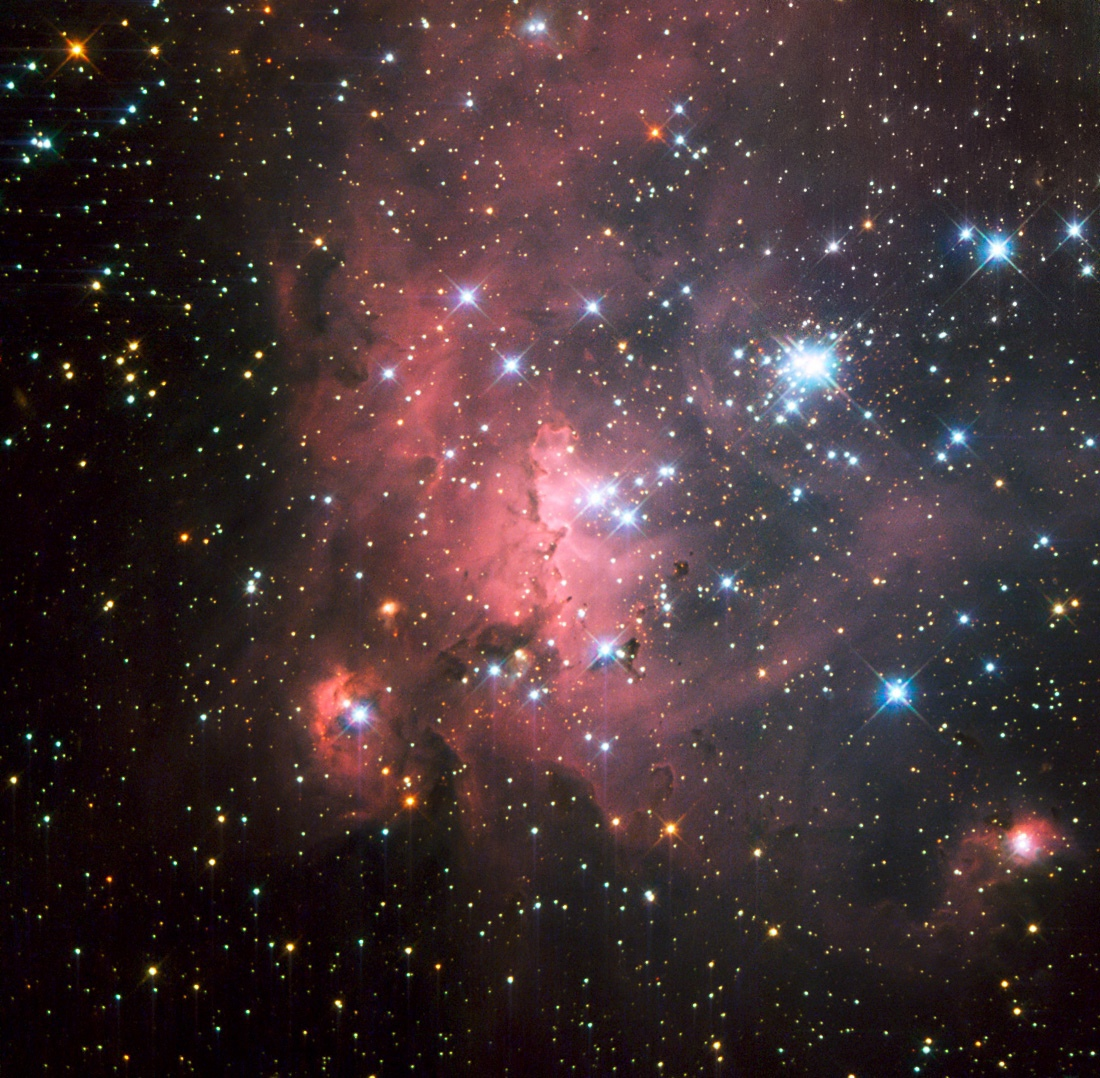
\includegraphics[width=0.4\textwidth]{pictures/Ass1.jpg}
            \caption{Трапеция Ориона}
        \end{figure}
    \end{frame}
    \begin{frame}
        Звёздные ассоциации впервые обнаружил Виктор Амбарцумян в 1947~г. и рассчитал, что такие объекты распадаются за несколько миллионов лет. 
        Это открытие также свидетельствовало о том, что звездообразование в Галактике происходит до сих пор.
        \begin{figure}
            \centering
            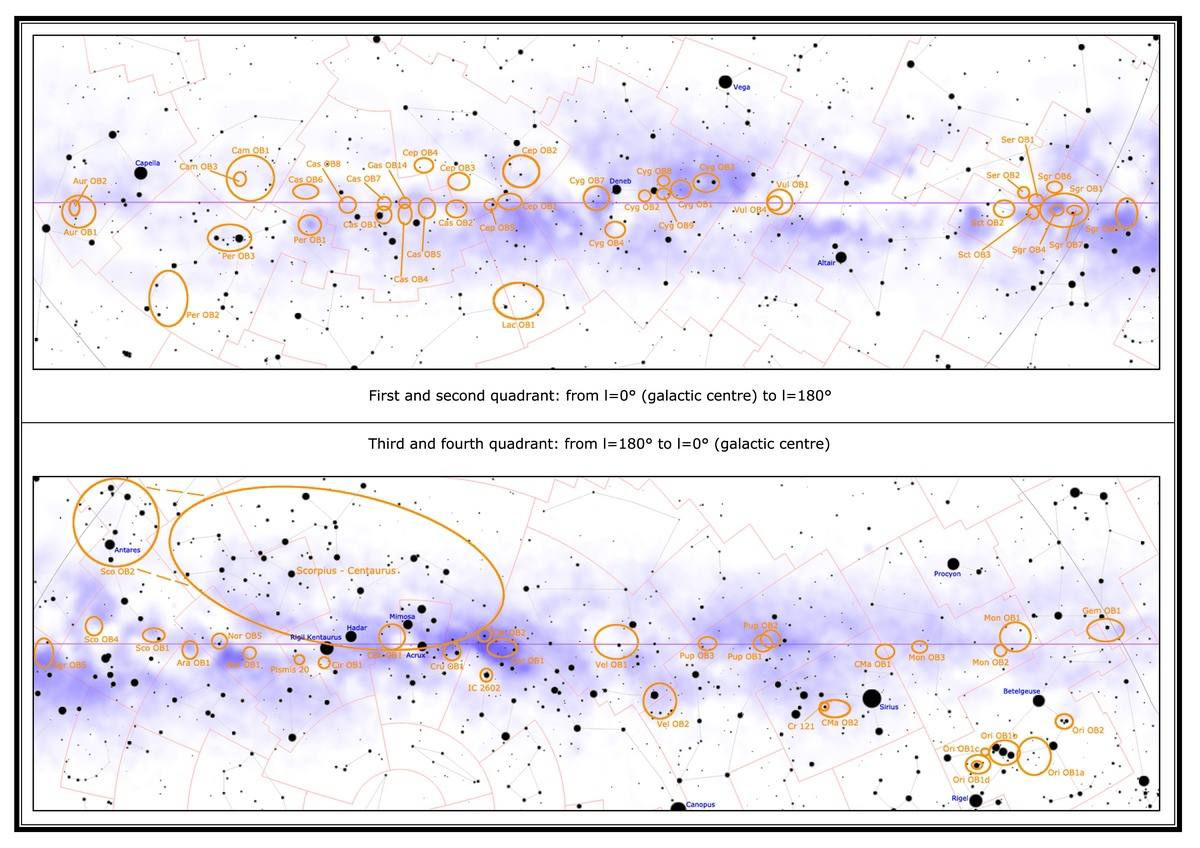
\includegraphics[width=0.6\textwidth]{pictures/Ass2.jpg}
        \end{figure}
    \end{frame}
    \subsection{Характеристики}
    \begin{frame}
        \begin{itemize}
            \item Отличия от РЗС:
            \begin{enumerate}
                \item Больший размер --- в~среднем $50$-$100$пк
                \item Меньшее количество --- в~звёздной ассоциации звёзд от~нескольких штук до~нескольких сотен
            \end{enumerate}
            \item Как правило, звёздные ассоциации находятся в~плоской составляющей диска Галактики толщиной $100$-$200$пк
            \item Звёзды имеют довольно маленький возраст (не более нескольких десятков миллионов лет)
            \item Содержание тяжёлых элементов в звездах довольно велико и составляет $2$-$3$\%
        \end{itemize}
    \end{frame}
    \subsection{Классификация}
    \begin{frame}
        Выделяют три типа звездных ассоциаций:
        \begin{itemize}
            \item OB-ассоциации также известные как O-ассоциации --- содержат массивные звёзды главной последовательности, 
            спектральных классов O и B
            \item T-ассоциации --- содержат в~основном маломассивные переменные звёзды типа Т Тельца, 
            ещё не дошедшие до~стадии главной последовательности
            \item R-ассоциации --- ассоциации, в~которых звёзды спектральных классов O-A2 окружены отражательными газопылевыми туманностями
        \end{itemize}
    \end{frame}

    %-------------------------------------------------------------------------------------
    \section{Список литературы}
    \begin{frame}[t, allowframebreaks]{Список литературы}
        \bibliographystyle{plain}
        \bibliography{bibliography}
    \end{frame}
\end{document}